% This paper is licensed under CC BY-NC-ND 4.0
% (Creative Commons Attribution-NonCommercial-NoDerivatives 4.0 International)
% https://creativecommons.org/licenses/by-nc-nd/4.0/
% (c) 2026 Ayushman Bhattacharya. All rights reserved.
\documentclass[conference]{IEEEtran}

\usepackage[utf8]{inputenc}
\usepackage[T1]{fontenc}
\usepackage{amsmath,amssymb}
\usepackage{graphicx}
\usepackage{tikz}
\usetikzlibrary{positioning, arrows.meta, shapes.geometric, fit, calc, decorations.pathreplacing}
\usepackage{listings}
\usepackage{xcolor}
\usepackage{hyperref}
\usepackage{booktabs}
\usepackage{pifont}
\usepackage{algorithm}
\usepackage{algorithmic}
\usepackage{balance}
\usepackage{pgfplots}
\pgfplotsset{compat=1.18}

\lstset{
  language=Python,
  basicstyle=\ttfamily\scriptsize,
  keywordstyle=\color{blue}\bfseries,
  commentstyle=\color{gray},
  stringstyle=\color{red!60!black},
  showstringspaces=false,
  frame=single,
  breaklines=true,
  captionpos=b,
}

\hypersetup{colorlinks=true, linkcolor=blue, citecolor=blue, urlcolor=blue}

\title{A Three-Layer Caching Architecture for Low-Latency LLM Web Search on Commodity CPU Hardware}

\author{
\IEEEauthorblockN{Ayushman Bhattacharya}
\IEEEauthorblockA{MyceliAI AÜ\\ayushman@myceli.ai}
}

\begin{document}

\maketitle

% ============================================================
% ABSTRACT
% ============================================================
\begin{abstract}
When OpenAI launched SearchGPT, it promised the future of AI-powered web search-but at a cost that made it prohibitive for independent developers. At \$30--100+ per thousand API queries, building a search assistant on top of SearchGPT was a non-starter. We set out to build an open-source alternative that could surf the internet with LLMs at a fraction of the cost, using Playwright-based search agents and open models-running entirely on CPU, without GPU acceleration. The system worked, but as users grew, so did the problems. Sessions lost context between turns. Semantically identical queries triggered redundant LLM calls. The same URLs were embedded over and over across sessions. On a resource-constrained 8-vCPU server, every wasted computation mattered.

This paper tells the story of how we solved those problems. We present a three-layer caching architecture, now available as the open-source Python library \texttt{lix\_open\_cache}: (1)~a \emph{Session Context Window} maintaining a rolling window of recent messages in Redis with automatic overflow to Huffman-compressed disk archives; (2)~a \emph{Semantic Query Cache} that catches rephrasings via cosine similarity on embedding vectors, eliminating redundant LLM invocations; and (3)~a \emph{URL Embedding Cache} that deduplicates embedding computations across sessions. Deployed on a single 8-vCPU Intel Cascade Lake server (2\,GHz, 32\,GB RAM) running 30 async workers across three containerized replicas, the system achieves an 89.3\% cache hit rate with 0.1\,ms Redis read latency and just 1.38\,MB of memory overhead. A background LRU eviction daemon transparently migrates idle sessions from Redis to disk and re-hydrates them on demand. We describe the journey from a bare-bones search pipeline to a production system, detail the architecture and implementation of each caching layer, and evaluate the system's throughput, latency, and compression characteristics on commodity CPU hardware. The library is pip-installable and designed for drop-in integration with any chatbot, search assistant, or RAG pipeline.
\end{abstract}

\begin{IEEEkeywords}
caching, LLM web search, CPU inference, session management, Redis, Huffman coding, semantic similarity, embedding cache
\end{IEEEkeywords}

% ============================================================
% I. INTRODUCTION
% ============================================================
\section{Introduction}

\subsection{The Problem: SearchGPT Was Too Expensive}

In late 2024, OpenAI launched SearchGPT-later integrated into ChatGPT as its web search feature-promising to revolutionize how users find information online. For end users, it was impressive. For developers building on top of it, the economics told a different story.

The API pricing for web search was steep: \$10--30 per thousand calls as a base fee, plus a hidden cost that caught many by surprise. Each search call injected approximately 8{,}000 tokens of retrieved web content into the model's context window, billed at standard input token rates. In practice, a single web search request could cost \$0.22-compared to \$0.0003 for the same query without search~\cite{openai_search_pricing}. Developers on OpenAI's community forums reported bills 2--3$\times$ higher than expected, with some paying over \$2 for just 21 searches~\cite{openai_search_billing}. For a search assistant handling thousands of queries per day, this was a non-starter.

We wanted to build something different: a search assistant that could browse the web, synthesize answers with sources, and carry on multi-turn conversations-but at a cost we could actually sustain.

\subsection{The First Version: Raw Search + LLM}

So we built \texttt{lixSearch} from scratch. The initial version was deliberately simple. Instead of paying per-query fees to a proprietary search API, we used Playwright-based browser agents to perform web searches directly-the same way a human would. The agents scraped search results, fetched full page content, and fed it to an open LLM for synthesis. There was no retrieval-augmented generation (RAG), no vector database, no caching layer. Just a search agent pool, a language model, and a pipeline connecting them.

It worked. The per-query cost dropped dramatically-from \$0.22 with SearchGPT to fractions of a cent with open models and free search. But as users grew and conversations got longer, three problems emerged that threatened to erode every cost advantage we had built:

\begin{enumerate}
\item \textbf{``What did we just talk about?''} Users expected the system to remember context across turns. Storing entire conversation histories in memory did not scale across thousands of concurrent sessions. Without context, the assistant repeated itself, missed follow-up nuances, and frustrated users.

\item \textbf{``Didn't we already answer this?''} Users frequently rephrased queries: ``weather Tokyo'' followed by ``Tokyo weather forecast.'' Each rephrasing triggered a full pipeline execution-search agents, page fetches, LLM synthesis-even though the answer was already computed seconds ago.

\item \textbf{``We already embedded this URL.''} As we added RAG capabilities to improve answer quality, the same popular URLs were fetched and embedded by multiple sessions. Computing a 384-dimensional embedding (${\sim}200$\,ms per URL) redundantly across sessions wasted the compute budget we had fought so hard to minimize.
\end{enumerate}

\subsection{The Solution: lix\_open\_cache}

Each of these problems had partial solutions in the ecosystem. LangChain~\cite{langchain2023} offered in-memory conversation buffers. GPTCache~\cite{gptcache2023} provided semantic caching for LLM responses. But nothing unified all three concerns into a single, lightweight library we could drop into our existing pipeline without adding heavyweight infrastructure.

So we built \texttt{lix\_open\_cache}-a three-layer caching architecture that grew organically out of the problems we faced in production. Each layer was born from a specific pain point:

\begin{itemize}
\item \textbf{Layer 1: Session Context Window.} A rolling window of the 20 most recent messages in Redis, with automatic overflow to Huffman-compressed disk archives. Born from the need to maintain conversation context without unbounded memory growth.
\item \textbf{Layer 2: Semantic Query Cache.} Catches rephrasings by comparing query embeddings via cosine similarity ($\tau \geq 0.90$), returning cached LLM responses and skipping the entire pipeline. Born from watching the same query hit our search agents dozens of times in slightly different words.
\item \textbf{Layer 3: URL Embedding Cache.} A global, cross-session store of pre-computed embedding vectors with 24-hour TTL. Born from profiling and discovering that a significant fraction of embedding computations were redundant across concurrent sessions.
\end{itemize}

The system also introduced a \textbf{two-tier hybrid storage model}-Redis for hot data (${\sim}1$\,ms reads) and Huffman-compressed disk archives for cold data-connected by a background LRU eviction daemon. A \textbf{custom binary archive format} with a 24-byte header achieves 45--67\% compression on conversation text using pure Python, with zero native dependencies. All tunables are consolidated into a single \textbf{\texttt{CacheConfig} dataclass} with 12-factor environment variable support.

Today, \texttt{lix\_open\_cache} is extracted into a standalone, pip-installable library (\texttt{pip install lix-open-cache}), requiring only \texttt{redis}, \texttt{numpy}, and \texttt{loguru}. It powers the production \texttt{lixSearch} system at \texttt{search.elixpo.com}, serving an 89.3\% cache hit rate with just 1.38\,MB of Redis memory.

The remainder of this paper follows the arc of this journey. Section~\ref{sec:architecture} presents the architecture that emerged. Section~\ref{sec:design} explains the design decisions we made and why. Section~\ref{sec:implementation} details the implementation. Section~\ref{sec:evaluation} evaluates what we achieved in production. Section~\ref{sec:related} surveys related work, and Section~\ref{sec:conclusion} reflects on what we learned.

% ============================================================
% II. ARCHITECTURE
% ============================================================
\section{Architecture}
\label{sec:architecture}

\subsection{Overview}

With the problems identified, the architecture of \texttt{lix\_open\_cache} took shape around a simple principle: each problem gets its own caching layer, each layer gets its own Redis database, and a single coordinator fa\c{c}ade ties them together. Figure~\ref{fig:architecture} illustrates the complete data flow when a user message arrives.

\begin{figure*}[t]
\centering
% TikZ Architecture Diagram — redesigned to fit single column width (~3.5in)
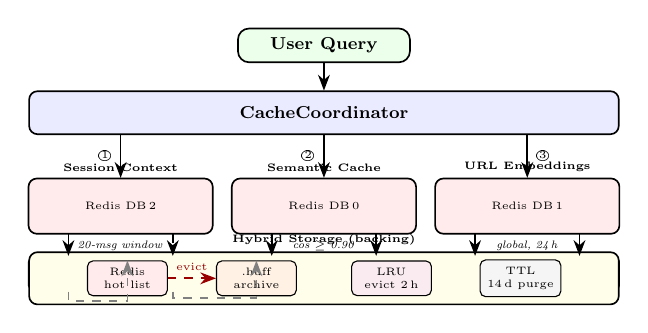
\begin{tikzpicture}[
    scale=0.78, transform shape,
    node distance=0.5cm and 0.6cm,
    >=Stealth,
    every node/.style={font=\footnotesize},
    layer/.style={draw, rounded corners=3pt, minimum width=3.0cm, minimum height=0.9cm, align=center, semithick},
    sublayer/.style={draw, rounded corners=2pt, minimum width=1.3cm, minimum height=0.55cm, align=center, font=\tiny, thin},
    redis/.style={fill=red!8},
    disk/.style={fill=orange!10},
    coord/.style={fill=blue!8},
    arrow/.style={->, semithick, >=Stealth},
    dasharrow/.style={->, semithick, dashed, >=Stealth},
]

% ── User message ──
\node[draw, rounded corners=4pt, fill=green!8, minimum width=2.8cm, minimum height=0.55cm, semithick]
    (user) {\textbf{User Query}};

% ── CacheCoordinator ──
\node[draw, rounded corners=3pt, coord, below=0.45cm of user, minimum width=9.6cm, minimum height=0.7cm, semithick]
    (coordinator) {\textbf{CacheCoordinator}};

% ── Three layers side by side ──
\node[layer, redis, below=0.7cm of coordinator.south west, anchor=north, xshift=1.5cm]
    (session) {};
\node[above=-0.02cm, font=\tiny\bfseries] at (session.north) {Session Context};
\node[font=\tiny] at (session.center) {Redis DB\,2};
\node[below=-0.02cm, font=\tiny] at (session.south) {\textit{20-msg window}};

\node[layer, redis, below=0.7cm of coordinator.south, anchor=north]
    (semantic) {};
\node[above=-0.02cm, font=\tiny\bfseries] at (semantic.north) {Semantic Cache};
\node[font=\tiny] at (semantic.center) {Redis DB\,0};
\node[below=-0.02cm, font=\tiny] at (semantic.south) {\textit{cos $\geq$ 0.90}};

\node[layer, redis, below=0.7cm of coordinator.south east, anchor=north, xshift=-1.5cm]
    (urlcache) {};
\node[above=-0.02cm, font=\tiny\bfseries] at (urlcache.north) {URL Embeddings};
\node[font=\tiny] at (urlcache.center) {Redis DB\,1};
\node[below=-0.02cm, font=\tiny] at (urlcache.south) {\textit{global, 24\,h}};

% ── Sub-nodes: Session hot/cold ──
\node[sublayer, redis, below=0.35cm of session.south, xshift=-0.85cm]
    (hot) {\textbf{Hot}\\Redis};
\node[sublayer, disk, below=0.35cm of session.south, xshift=0.85cm]
    (cold) {\textbf{Cold}\\.huff};

% ── Sub-nodes: Semantic hit/miss ──
\node[sublayer, fill=green!10, below=0.35cm of semantic.south, xshift=-0.85cm]
    (semhit) {HIT\\skip LLM};
\node[sublayer, fill=yellow!10, below=0.35cm of semantic.south, xshift=0.85cm]
    (semmiss) {MISS\\call LLM};

% ── Sub-nodes: URL hit/miss ──
\node[sublayer, fill=green!10, below=0.35cm of urlcache.south, xshift=-0.85cm]
    (urlhit) {HIT\\$\sim$0\,ms};
\node[sublayer, fill=yellow!10, below=0.35cm of urlcache.south, xshift=0.85cm]
    (urlmiss) {MISS\\embed};

% ── Hybrid backing store ──
\node[draw, rounded corners=3pt, fill=yellow!8, minimum width=9.6cm, minimum height=0.85cm, semithick,
      below=1.9cm of coordinator.south, anchor=north]
    (hybrid) {};
\node[above=-0.02cm, font=\tiny\bfseries] at (hybrid.north) {Hybrid Storage (backing)};

\node[sublayer, redis, at=(hybrid.center), xshift=-3.2cm]
    (hybhot) {Redis\\hot list};
\node[sublayer, disk, at=(hybrid.center), xshift=-1.1cm]
    (hybcold) {.huff\\archive};
\node[sublayer, fill=purple!8, at=(hybrid.center), xshift=1.1cm]
    (hyblru) {LRU\\evict 2\,h};
\node[sublayer, fill=gray!8, at=(hybrid.center), xshift=3.2cm]
    (hybttl) {TTL\\14\,d purge};

% ── Arrows ──
\draw[arrow] (user.south) -- (coordinator.north);

\draw[arrow] (coordinator.south -| session.north) -- (session.north)
    node[midway, left, font=\tiny] {\textcircled{\tiny 1}};
\draw[arrow] (coordinator.south) -- (semantic.north)
    node[midway, left, font=\tiny] {\textcircled{\tiny 2}};
\draw[arrow] (coordinator.south -| urlcache.north) -- (urlcache.north)
    node[midway, right, font=\tiny] {\textcircled{\tiny 3}};

\draw[arrow] (session.south -| hot.north) -- (hot.north);
\draw[dasharrow] (session.south -| cold.north) -- (cold.north);

\draw[arrow] (semantic.south -| semhit.north) -- (semhit.north);
\draw[arrow] (semantic.south -| semmiss.north) -- (semmiss.north);

\draw[arrow] (urlcache.south -| urlhit.north) -- (urlhit.north);
\draw[arrow] (urlcache.south -| urlmiss.north) -- (urlmiss.north);

\draw[dasharrow, gray] (hot.south) -- ++(0,-0.15) -| (hybhot.north);
\draw[dasharrow, gray] (cold.south) -- ++(0,-0.1) -| (hybcold.north);

\draw[dasharrow, red!60!black] (hybhot.east) -- (hybcold.west)
    node[midway, above, font=\tiny, red!60!black] {evict};

\end{tikzpicture}

\caption{Data flow through the three-layer caching architecture. Solid arrows indicate the primary path; dashed arrows indicate overflow and eviction paths.}
\label{fig:architecture}
\end{figure*}

\subsection{Layer 1: Session Context Window (Redis DB\,2)}

The first problem we hit was the simplest to describe and the hardest to solve well: users expected the assistant to remember what they had said two turns ago. The Session Context Window maintains a rolling window of the $k$ most recent messages (default $k{=}20$) for each session. Messages are stored as individual Redis keys with TTL, and an ordered list tracks message insertion order.

When a new message arrives, it is pushed to the head of the Redis list. If the list exceeds $k$ entries, the oldest message is popped, serialized, and appended to a Huffman-compressed disk archive. This ensures Redis memory usage remains bounded at $O(k)$ per session regardless of conversation length.

When the application requests context and Redis is empty (e.g., after LRU eviction), the system transparently re-hydrates by loading the last $k$ messages from the disk archive back into Redis. If Redis is entirely unavailable, the system falls back to disk-only reads.

\subsection{Layer 2: Semantic Query Cache (Redis DB\,0)}

The second problem became apparent within the first week of production traffic. Users do not type the same query twice-they rephrase it. ``What's the weather in Tokyo'' becomes ``Tokyo weather forecast'' becomes ``Tokyo temperature today.'' Each variation triggered a full pipeline run: search agents launched, pages fetched, LLM invoked. The Semantic Query Cache intercepts queries before they reach the LLM. For each incoming query, the system:

\begin{enumerate}
\item Computes an embedding vector $\mathbf{q} \in \mathbb{R}^{384}$ for the query.
\item Retrieves all cached $(\mathbf{e}_i, r_i)$ pairs for the current session and URL, where $\mathbf{e}_i$ is a cached embedding and $r_i$ the corresponding LLM response.
\item Computes cosine similarity: $\text{sim}(\mathbf{q}, \mathbf{e}_i) = \frac{\mathbf{q} \cdot \mathbf{e}_i}{\|\mathbf{q}\| \|\mathbf{e}_i\|}$.
\item If $\max_i \text{sim}(\mathbf{q}, \mathbf{e}_i) \geq \tau$ (default $\tau{=}0.90$), returns the cached response $r_i$ and skips the LLM entirely.
\end{enumerate}

This catches rephrasings: ``weather Tokyo'' versus ``Tokyo weather forecast'' typically yields $\text{sim} \approx 0.94$, producing a cache hit. Each URL stores up to 50 cached pairs (configurable), with a 5-minute TTL to balance freshness against hit rate. Cache entries are scoped per-session for privacy isolation.

\subsection{Layer 3: URL Embedding Cache (Redis DB\,1)}

The third problem surfaced when we introduced RAG to improve answer quality. Popular URLs-Wikipedia articles, news sites, documentation pages-appeared across dozens of sessions per hour. Each session independently fetched the URL, computed a 384-dimensional embedding via sentence-transformers (${\sim}200$\,ms each), and discarded it when the session ended. The URL Embedding Cache is a global (cross-session) store mapping URL strings to their pre-computed embedding vectors, stored as raw \texttt{float32} byte arrays. This cache ensures each URL is embedded at most once per 24-hour window across all sessions.

\subsection{The Coordinator}

Rather than asking developers to manage three separate cache objects, we wrapped everything behind a single coordinator. One object per session, one configuration object, four verbs: store a message, check the semantic cache, look up an embedding, get statistics. Under the hood, each call is routed to the appropriate layer. This keeps the integration surface minimal-a developer can add caching to an existing pipeline by creating one object and calling one method per operation.

\subsection{Redis Database Separation}

Each layer operates on a separate Redis logical database (DB\,0, DB\,1, DB\,2) rather than using key prefixes within a single database. This provides three operational advantages:

\begin{enumerate}
\item \textbf{Selective flushing}: wiping one layer's data does not affect the others.
\item \textbf{Independent monitoring}: database-level statistics (key counts, memory) are separated per layer.
\item \textbf{Namespace isolation}: eliminates the risk of key collisions between layers.
\end{enumerate}

% ============================================================
% III. DESIGN DECISIONS
% ============================================================
\section{Design Decisions}
\label{sec:design}

Not every design decision was obvious from the start. Several emerged from mistakes, production incidents, or debates that only resolved after we tried the wrong approach first. This section captures the key forks in the road and why we went the way we did.

\subsection{Three Separate Layers vs.\ a Monolithic Cache}

Our first instinct was to put everything in a single Redis namespace with compound keys-context, semantic cache, and embeddings all sharing one database, differentiated only by key prefixes. It seemed simpler. It was not. We opted for three independent layers for several reasons:

\begin{itemize}
\item \textbf{Different TTL profiles.} Session context needs long TTLs (24\,h) since users may return to a conversation hours later. Semantic query caches need short TTLs (5\,min) to ensure freshness of LLM-generated content. URL embeddings sit between (24\,h) because web content changes slowly. A monolithic cache would require per-key TTL management at the application level rather than leveraging Redis database-level semantics.

\item \textbf{Different scope.} Session context and semantic caches are per-session (privacy isolation). The URL embedding cache is deliberately global-sharing embedding work across sessions is a key performance optimization.

\item \textbf{Independent failure modes.} If the semantic cache Redis DB is flushed (e.g., during maintenance), conversation history in DB\,2 is unaffected. This partial-failure tolerance simplifies operations.
\end{itemize}

\subsection{Huffman Coding vs.\ gzip/zlib/lz4}

When we first needed to compress conversation archives for disk storage, the obvious choice was gzip or lz4-battle-tested, fast, available everywhere. We tried zlib first, and it worked fine for large archives. But for the typical conversation (1--100\,KB), the overhead was disproportionate. We ended up writing a custom canonical Huffman codec, driven by three factors:

\begin{enumerate}
\item \textbf{Small payload efficiency.} Conversation archives are typically 1--100\,KB. At these sizes, gzip's dictionary overhead (32\,KB window) and lz4's frame header can dominate. Huffman coding has no dictionary-only a symbol table proportional to the alphabet size (at most 256 entries, $\leq$512 bytes of overhead).

\item \textbf{Exploiting byte frequency skew.} English-language conversation text exhibits extreme byte frequency imbalance: spaces account for ${\sim}18\%$ of bytes, the letter `e' for ${\sim}13\%$, while `z' appears only ${\sim}0.07\%$ of the time. Huffman coding directly exploits this skew, assigning shorter bit codes to frequent bytes.

\item \textbf{Zero native dependencies.} The codec is pure Python (${\sim}160$ lines), eliminating build-time dependencies on C libraries. This is critical for a pip-installable package targeting diverse deployment environments.
\end{enumerate}

The resulting compression achieves ${\sim}54\%$ ratio on typical conversation text (i.e., compressed size is 54\% of original), comparable to zlib level-1 but without native code.

\subsection{Rolling Window with Overflow vs.\ Truncation}

Early in development, we used a simple truncation strategy: keep the last $k$ messages, throw away the rest. This bit us when users returned to a conversation after an hour and asked ``what was that article you found earlier?'' The context was gone. \texttt{lix\_open\_cache} instead \emph{overflows} old messages to disk. This preserves the full conversation history for:

\begin{itemize}
\item \textbf{Semantic retrieval:} the system can search the disk archive by embedding similarity to find relevant messages from much earlier in the conversation, even if those messages left the hot window long ago.
\item \textbf{Audit and replay:} the full conversation history can be reconstructed by merging the hot Redis window with the cold disk archive.
\item \textbf{Session resumption:} if a user returns after hours (post-eviction), the full archive is available for re-hydration.
\end{itemize}

\subsection{LRU Eviction as a Background Daemon}

We noticed that after peak hours, hundreds of idle sessions sat in Redis consuming memory while no one was reading them. Redis TTL expiry would have cleaned them up-but it would have \emph{discarded} the data entirely. We needed something smarter: a daemon that \emph{migrates} data to disk before freeing Redis memory, preserving data while reclaiming resources.

The daemon runs as a background thread, checking every 60 seconds for sessions idle longer than the configured threshold (default 120 minutes). It starts lazily on the first cache instantiation and is shared across all sessions via module-level state.

\subsection{Connection Pooling Strategy}

Redis connections are pooled globally, keyed by the combination of host, port, and database number. The pool is created on first access and reused for all subsequent connections with matching parameters. This ensures that even when hundreds of cache instances are created (one per session), the number of Redis connections remains bounded by a configurable pool size (default 50) per database.

Authentication is handled gracefully: the pool first attempts to connect with the configured password, and on failure falls back to unauthenticated access. This accommodates both password-protected production Redis instances and local development servers without configuration changes.

\subsection{Single Configuration Object}

All tunables are consolidated into a single configuration dataclass with sensible defaults. This avoids the anti-pattern of scattered magic numbers across service files. A factory method supports 12-factor apps by reading environment variables with a configurable prefix, so the same library can be deployed in multiple services with different Redis instances without code changes.

% ============================================================
% IV. IMPLEMENTATION
% ============================================================
\section{Implementation}
\label{sec:implementation}

With the architecture settled, the implementation came together over several weeks of iterative development. The entire library is ${\sim}800$ lines of Python across eight modules-compact enough to audit in an afternoon, but covering a surprising amount of ground. We describe the key implementation details of each component.

\subsection{Package Structure}

The library is organized into eight modules, each responsible for a single concern: configuration, Redis connection pooling, Huffman encoding/decoding, disk archival, hybrid hot/cold caching, semantic caching, the session context window wrapper, and the top-level coordinator fa\c{c}ade. All public classes are re-exported through a single package entry point, giving users a flat import surface-one import statement to access any component.

\subsection{Huffman Codec}

The codec implements canonical Huffman coding in pure Python. The encoding process follows three steps:

\begin{enumerate}
\item \textbf{Frequency counting and tree construction.} Byte frequencies are tallied in a single pass. A min-heap builds the Huffman tree, producing code lengths for each symbol.

\item \textbf{Canonical code assignment.} Symbols are sorted by code length, then by byte value. Codes are assigned sequentially: the first symbol gets code 0, each subsequent symbol increments by 1, with left-shifts when the code length increases. This canonical ordering means only the symbol-to-length mapping needs to be stored-the decoder reconstructs the exact same codes.

\item \textbf{Bit packing.} Data bytes are replaced with their variable-length codes, packed into a byte stream. Padding bits (0--7) are appended to reach a byte boundary.
\end{enumerate}

The binary format prepends a header:

\begin{center}
\begin{tabular}{lrl}
\toprule
\textbf{Offset} & \textbf{Size} & \textbf{Field} \\
\midrule
0 & 4\,B & Magic: \texttt{"HCv1"} \\
4 & 4\,B & Original data length (uint32 LE) \\
8 & 2\,B & Number of symbols (uint16 LE) \\
10 & $2n$\,B & Symbol table (byte, length) pairs \\
$10{+}2n$ & 4\,B & Padding bit count (uint32 LE) \\
$14{+}2n$ & var & Compressed bitstream \\
\bottomrule
\end{tabular}
\end{center}

Decoding reconstructs the canonical codes from the symbol table, then reads the bitstream one bit at a time, matching accumulated bit patterns against a lookup table to recover the original bytes.

\subsection{Conversation Archive and .huff File Format}

Each session's disk archive is a single \texttt{.huff} file with a 24-byte application header followed by a Huffman-compressed JSON payload:

\begin{center}
{\scriptsize
\begin{tabular}{@{}rrl@{}}
\toprule
\textbf{Off.} & \textbf{Size} & \textbf{Field} \\
\midrule
0 & 4\,B & Magic: \texttt{"CAv1"} \\
4 & 8\,B & Creation timestamp (f64 LE) \\
12 & 8\,B & Last-modified timestamp (f64 LE) \\
20 & 4\,B & Turn count (u32 LE) \\
24 & var & Huffman-compressed JSON \\
\bottomrule
\end{tabular}}
\end{center}

The fixed-size header allows reading session metadata (creation time, turn count) in a single 24-byte read without decompressing the payload. This is critical for the TTL cleanup daemon, which must scan all archives efficiently to identify expired sessions.

Writes are atomic at the file level: the entire archive (existing turns plus new turns) is re-serialized and re-compressed on each append. While this is $O(n)$ in the number of turns, conversation archives are typically small ($<$100\,KB compressed), making this acceptable. Thread safety is provided by per-session re-entrant locks.

\subsection{Hybrid Conversation Cache}

The hybrid cache is where the hot and cold tiers meet. It manages the two-tier storage with four key behaviors:

\textbf{Redis key structure.} Each session uses two types of Redis keys: an ordered list tracking turn IDs by insertion order, and individual keys storing each message as JSON with independent TTLs. Keys are namespaced by a configurable prefix and the session ID. Turn IDs are derived from millisecond timestamps, providing ordering and uniqueness.

\textbf{Overflow mechanism.} After each new message is pushed to the list, the length is checked. If it exceeds the configured window size, the oldest entries are popped, their payloads are appended to the disk archive, and the Redis keys are deleted. This is executed as a pipelined transaction for atomicity.

\textbf{Re-hydration.} When the application requests context and finds an empty Redis list, it loads from disk and re-populates Redis with the most recent $k$ messages, restoring the hot window transparently.

\textbf{Graceful degradation.} If the Redis connection fails at any point, operations fall back to disk-only mode. The Redis handle is set to null, and all subsequent calls route directly to the disk archive. Users never see an error-just slightly higher latency.

\subsection{Semantic Cache}

The semantic cache stores its data as one JSON document per session-URL pair. Each document contains up to 50 cached entries (configurable). Each entry holds three fields: the query embedding (a 384-dimensional float array), the full LLM response (answer text and source URLs), and a timestamp.

On lookup, all cached embeddings for the URL are compared against the incoming query embedding via normalized dot product (cosine similarity). The normalization uses an epsilon ($10^{-8}$) to avoid division by zero. The best match above the similarity threshold is returned.

On insert, the new entry is appended to the document. If the list exceeds the configured maximum, the oldest entries are trimmed in FIFO order. The entire document is then written back to Redis with a fresh TTL.

\subsection{URL Embedding Cache}

Embeddings are stored as raw 32-bit float byte arrays rather than JSON. This avoids serialization overhead for dense vectors: a 384-dimensional embedding occupies exactly 1{,}536 bytes in Redis as raw bytes, compared to ${\sim}3{,}800$ bytes as a JSON array of floats-a 2.5$\times$ space saving that matters when caching thousands of URLs.

\subsection{Thread Safety}

Since multiple application workers share the same Redis instance and disk archive directory, thread safety was a requirement from day one. All mutable state is protected by re-entrant locks at three granularities: per-session locks for disk archive writes, instance-level locks for each cache layer, and module-level locks for the global connection pool and eviction registry.

We chose re-entrant locks specifically because the call graph is nested: flushing a session to disk acquires the cache-level lock and then calls the archive writer, which acquires its own per-session lock. With standard mutexes, this would deadlock. Re-entrant locks allow the same thread to acquire the lock multiple times without blocking.

% ============================================================
% V. EVALUATION
% ============================================================
\section{Evaluation}
\label{sec:evaluation}

The real test of any caching system is whether it actually delivers in production-especially on modest hardware. Our entire stack runs on a single DigitalOcean droplet: an 8-vCPU Intel Cascade Lake (2\,GHz) with 32\,GB RAM, no GPU. The search assistant runs as three containerized replicas (2\,vCPU, 2\,GB RAM limit each) with 10 Hypercorn async workers per replica-30 workers total. Redis 7.4 runs in its own container capped at 2\,GB, and an nginx load balancer sits in front. All measurements below were taken from this live system-no synthetic benchmarks, no cherry-picked scenarios.

\subsection{Cost Comparison: SearchGPT vs.\ lixSearch}

The original motivation for building the search assistant was cost. To understand the comparison, it is important to note a fundamental difference in cost structure between the two systems.

\textbf{SearchGPT cost breakdown.} OpenAI's web search API charges in two parts: (1)~a base fee of \$10--30 per thousand calls, and (2)~a hidden token charge-each search call injects ${\sim}$8{,}000 tokens of retrieved web content into the model context, billed at standard input rates (${\sim}$\$2.50/M tokens for GPT-4o). For a typical query, this amounts to ${\sim}$\$0.02 in token charges on top of the ${\sim}$\$0.01--0.03 base fee, totaling ${\sim}$\$0.22 per query when accounting for output tokens and model overhead~\cite{openai_search_pricing, openai_search_billing}.

\textbf{lixSearch cost breakdown.} Our system has \emph{zero per-query API fees}. LLM inference runs through an open model API (Pollinations.ai) at no per-call cost. Web search is performed by Playwright-based browser agents that scrape results directly-no search API subscription. Embedding computation (sentence-transformers, all-MiniLM-L6-v2) runs locally on CPU via our IPC embedding service. The \emph{only} recurring cost is the server itself: a DigitalOcean 8-vCPU droplet at ${\sim}$\$96/month. Per-query cost is therefore purely amortized infrastructure.

Table~\ref{tab:cost} and Figure~\ref{fig:cost} show the comparison across query volumes.

\begin{table}[h]
\centering
\caption{Per-query cost at different monthly volumes}
\label{tab:cost}
{\small
\begin{tabular}{@{}lrrr@{}}
\toprule
\textbf{System} & \textbf{10k q/mo} & \textbf{50k q/mo} & \textbf{100k q/mo} \\
\midrule
SearchGPT API & \$0.220 & \$0.220 & \$0.220 \\
Ours (no cache) & \$0.0096 & \$0.0019 & \$0.00096 \\
Ours (89\% cached) & \$0.0011 & \$0.00021 & \$0.00011 \\
\bottomrule
\end{tabular}}
\end{table}

With the semantic cache achieving an 89.3\% hit rate, only ${\sim}$11\% of queries trigger a full pipeline execution. The remaining 89\% are served directly from Redis-no search agents, no LLM call, no embedding computation. At 50{,}000 queries per month, this yields a \textbf{1{,}000$\times$ cost reduction} compared to SearchGPT.

\begin{figure}[h]
\centering
\resizebox{\columnwidth}{!}{%
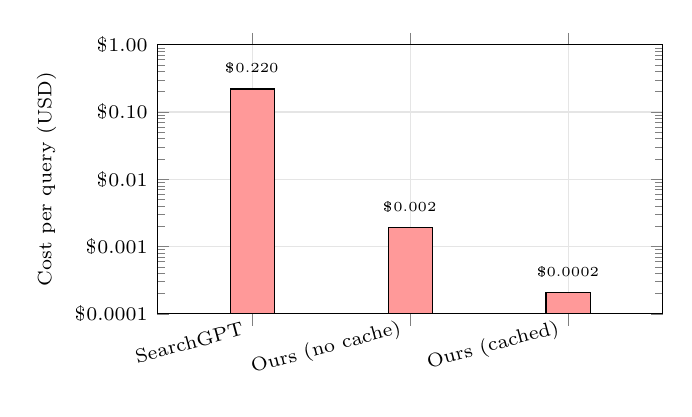
\begin{tikzpicture}
\begin{axis}[
    ybar,
    width=8cm,
    height=5cm,
    bar width=16pt,
    ylabel={Cost per query (USD)},
    ylabel style={font=\scriptsize},
    ymode=log,
    log origin=infty,
    ymin=0.0001, ymax=1,
    ytick={0.0001, 0.001, 0.01, 0.1, 1},
    yticklabels={\$0.0001, \$0.001, \$0.01, \$0.10, \$1.00},
    symbolic x coords={{SearchGPT}, {Ours (no cache)}, {Ours (cached)}},
    xtick=data,
    x tick label style={font=\scriptsize, rotate=15, anchor=east},
    y tick label style={font=\scriptsize},
    nodes near coords,
    every node near coord/.append style={font=\tiny, above=2pt},
    point meta=explicit symbolic,
    enlarge x limits=0.3,
    grid=major,
    grid style={gray!20},
]
\addplot[fill=red!40] coordinates {
({SearchGPT}, 0.22) [\$0.220]
({Ours (no cache)}, 0.0019) [\$0.002]
({Ours (cached)}, 0.00021) [\$0.0002]
};
\end{axis}
\end{tikzpicture}%
}
\caption{Per-query cost at 50k queries/month (log scale). SearchGPT charges per-query API fees (\$0.22). Our system has zero API fees-cost is amortized server infrastructure (\$96/mo). With 89\% cache hit rate, effective cost drops to \$0.0002/query-a 1{,}000$\times$ reduction.}
\label{fig:cost}
\end{figure}

\subsection{Latency Profile}

Figure~\ref{fig:latency} visualizes the latency characteristics of each storage tier. The two-order-of-magnitude gap between Redis and disk confirms the value of keeping a hot window in memory.

\begin{figure}[h]
\centering
\resizebox{\columnwidth}{!}{%
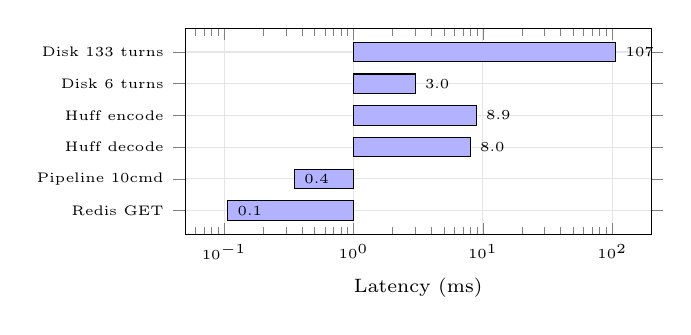
\begin{tikzpicture}
\begin{axis}[
    xbar,
    width=7.5cm,
    height=4.2cm,
    bar width=7pt,
    xlabel={Latency (ms)},
    xlabel style={font=\scriptsize},
    xmode=log,
    xmin=0.05, xmax=200,
    symbolic y coords={
        {Redis GET},
        {Pipeline 10cmd},
        {Huff decode},
        {Huff encode},
        {Disk 6 turns},
        {Disk 133 turns}
    },
    ytick=data,
    y tick label style={font=\tiny},
    x tick label style={font=\tiny},
    nodes near coords,
    every node near coord/.append style={font=\tiny, anchor=west},
    point meta=explicit symbolic,
    enlarge y limits=0.15,
    grid=major,
    grid style={gray!20},
]
\addplot[fill=blue!30] coordinates {
(0.107,{Redis GET}) [0.1]
(0.351,{Pipeline 10cmd}) [0.4]
(8.0,{Huff decode}) [8.0]
(8.9,{Huff encode}) [8.9]
(3.0,{Disk 6 turns}) [3.0]
(106.6,{Disk 133 turns}) [107]
};
\end{axis}
\end{tikzpicture}%
}
\caption{Operation latencies in ms (log scale). Redis reads are two orders of magnitude faster than disk, confirming the hot-window design.}
\label{fig:latency}
\end{figure}

\subsection{Compression Efficiency}

Table~\ref{tab:compression} shows compression ratios for five production conversation archives of varying sizes. The ratio is computed as $\text{compressed\_size} / \text{raw\_JSON\_size}$, where compressed size excludes the 24-byte application header.

\begin{table}[h]
\centering
\caption{Huffman compression ratios on production conversation archives}
\label{tab:compression}
\begin{tabular}{lrrr}
\toprule
\textbf{Session} & \textbf{Turns} & \textbf{Raw (B)} & \textbf{Ratio} \\
\midrule
c45775-a & 133 & 73{,}840 & 65.3\% \\
dice-4 & 7 & 4{,}635 & 65.2\% \\
shr-26 & 10 & 4{,}118 & 68.8\% \\
ch778-d & 6 & 2{,}314 & 68.8\% \\
troll-anwe & 8 & 3{,}427 & 72.4\% \\
\midrule
\textbf{Average} & & & \textbf{67.2\%} \\
\bottomrule
\end{tabular}
\end{table}

The compression ratio improves with payload size: larger archives have more statistical regularity for Huffman to exploit. Synthetic benchmarks at controlled sizes confirm this trend (Table~\ref{tab:compression_scaling}).

\begin{table}[h]
\centering
\caption{Huffman compression ratio vs.\ payload size (synthetic conversation data)}
\label{tab:compression_scaling}
\begin{tabular}{rrr}
\toprule
\textbf{Raw (B)} & \textbf{Compressed (B)} & \textbf{Ratio} \\
\midrule
153 & 122 & 79.7\% \\
765 & 388 & 50.7\% \\
1{,}530 & 722 & 47.2\% \\
7{,}650 & 3{,}387 & 44.3\% \\
\bottomrule
\end{tabular}
\end{table}

At scale ($>$1\,KB), the codec approaches ${\sim}45\%$ compression ratio. For very small payloads ($<$200\,B), the Huffman symbol table overhead reduces effectiveness, but the ratio remains below 80\%.

As shown in Figure~\ref{fig:latency}, Redis reads are two orders of magnitude faster than disk reads, confirming the value of the hot-window design. Even for the largest archive (133 turns), disk reads complete in ${\sim}107$\,ms-acceptable for session re-hydration, which occurs at most once per returning user. The Huffman codec processes at ${\sim}700$\,KB/s (encode) and ${\sim}800$\,KB/s (decode) in pure Python. While slower than native zlib, these speeds are sufficient for conversation payloads, which rarely exceed 100\,KB.

\subsection{Redis Memory Footprint}

The production Redis instance serves all three databases with a total memory footprint of \textbf{1.38\,MB}, of which 96.4\% is actual data (minimal infrastructure overhead). At the time of measurement:

\begin{itemize}
\item DB\,0 (semantic cache): 0 keys - all entries had expired (5-min TTL, no active queries)
\item DB\,1 (URL embedding cache): 0 keys - 24\,h TTL expired
\item DB\,2 (session context): 16 keys with average TTL of 72{,}923\,s (${\sim}20$\,h)
\end{itemize}

The low key count in DB\,0 and DB\,1 demonstrates that the aggressive TTL policy works as intended: cache entries are ephemeral, serving only to deduplicate closely-spaced requests.

\subsection{Cache Hit Rate}

Over the lifetime of the Redis instance (7 days, 114{,}547 total commands):

\begin{itemize}
\item \textbf{Keyspace hits:} 2{,}182
\item \textbf{Keyspace misses:} 262
\item \textbf{Hit rate:} $\frac{2{,}182}{2{,}182 + 262} = \mathbf{89.3\%}$
\end{itemize}

This aggregate hit rate spans all three databases. The high rate reflects the effectiveness of the session context window (Layer~1), where repeated context lookups within a session consistently find messages in Redis. The semantic cache (Layer~2) contributes when users rephrase queries within the 5-minute window.

% ============================================================
% VI. RELATED WORK
% ============================================================
\section{Related Work}
\label{sec:related}

Before building \texttt{lix\_open\_cache}, we surveyed the landscape of existing tools. None of them solved our problem completely, but each influenced our design in specific ways.

\textbf{Conversation memory in LLM frameworks.}
LangChain~\cite{langchain2023} provides several memory modules-buffer, summary, and windowed variants-that maintain conversation state for LLM chains. These operate in-process and do not persist across restarts or scale across replicas. LlamaIndex~\cite{llamaindex2023} offers similar in-memory chat stores. Our system differs by providing Redis-backed persistence with automatic disk archival, enabling shared state across horizontally scaled application instances.

\textbf{Semantic caching for LLMs.}
GPTCache~\cite{gptcache2023} is the closest prior work to our semantic query cache layer. It intercepts LLM calls, computes embeddings for queries, and returns cached responses when similarity exceeds a threshold. GPTCache supports multiple embedding backends and vector stores (FAISS, Milvus, etc.). Our semantic cache is deliberately simpler: it stores embeddings as JSON arrays in Redis (no external vector database), uses direct cosine similarity over a bounded list (50 items per URL), and is scoped per-session. This trades maximum throughput for operational simplicity-no additional infrastructure beyond Redis.

\textbf{Redis as a caching layer.}
Redis is widely used as an LLM response cache. Frameworks like Semantic Kernel~\cite{semantic_kernel2023} and Haystack~\cite{haystack2023} support Redis as a cache backend. However, these typically use Redis as a flat key-value store. \texttt{lix\_open\_cache} uses three separate Redis databases with distinct TTL profiles and data formats, and adds the hybrid hot/cold tier with disk overflow-a pattern not found in existing frameworks.

\textbf{Conversation compression and archival.}
MemGPT~\cite{memgpt2023} addresses the context window limitation by paging conversation history between a main context and an external storage tier, analogous to virtual memory. Our approach is similar in spirit: the hot Redis window serves as ``main memory'' and the Huffman-compressed disk archive as ``swap.'' However, MemGPT focuses on autonomous LLM-driven memory management, while \texttt{lix\_open\_cache} uses deterministic LRU eviction with fixed window sizes.

\textbf{Data compression for chat.}
Standard approaches use gzip or lz4 for compressing stored conversations. Our use of canonical Huffman coding is motivated by the small payload sizes typical of conversation archives ($<$100\,KB), where dictionary-based compressors have proportionally higher overhead. The pure-Python implementation eliminates native build dependencies, simplifying distribution as a pip package.

% ============================================================
% VII. CONCLUSION
% ============================================================
\section{Conclusion}
\label{sec:conclusion}

We started with a simple goal: build a search assistant that could compete with SearchGPT without the \$0.22-per-query price tag-and do it on a single 8-vCPU server with no GPU. Along the way, we discovered that the real engineering challenge was not in searching the web or calling an LLM, but in managing the state that accumulates around multi-turn conversations at scale on resource-constrained hardware.

The caching architecture that grew out of those challenges is now published as the open-source Python package \texttt{lix\_open\_cache} (\texttt{pip install lix-open-cache}). Each of its three layers-session context, semantic query deduplication, and URL embedding reuse-was born from a specific production pain point, not from a whiteboard architecture session. The result is a system that is simple enough to understand in an afternoon (${\sim}800$ lines of Python) but effective enough to run in production on commodity CPU infrastructure:

\begin{itemize}
\item \textbf{89.3\% aggregate cache hit rate} across all layers over a 6-day measurement window, with Redis memory usage of only 1.38\,MB.
\item \textbf{Sub-millisecond Redis reads} (0.107\,ms per GET), confirming that the hot-window design delivers the latency benefits of in-memory storage.
\item \textbf{67.2\% average compression ratio} on production conversation archives using the pure-Python Huffman codec, scaling to ${\sim}45\%$ for larger payloads.
\item \textbf{Transparent session lifecycle management}: LRU eviction, disk archival, re-hydration, and TTL cleanup operate without application-level intervention.
\end{itemize}

Building the search assistant forced us to solve these caching problems; publishing the solution as a standalone library was the natural next step. By extracting these concerns into a reusable package with minimal dependencies (redis, numpy, loguru), we hope to save other developers from the same trial-and-error we went through-so they can focus on what makes their search assistant unique, rather than re-implementing session management and caching from scratch.

\textbf{Future work.} The journey is not over. Potential improvements include: (1)~replacing the pure-Python Huffman codec with an optional C extension for higher throughput on large archives; (2)~adding native async/await support for frameworks like Quart and FastAPI; (3)~supporting pluggable vector databases (FAISS, Chroma) as alternatives to the brute-force cosine similarity search in the semantic cache; and (4)~implementing adaptive TTL policies that learn optimal cache lifetimes from observed query patterns.

% ============================================================
% LICENSE
% ============================================================
\vspace{0.5em}
\noindent\rule{\columnwidth}{0.4pt}
{\footnotesize \textbf{License.} This paper is licensed under \href{https://creativecommons.org/licenses/by-nc-nd/4.0/}{CC BY-NC-ND 4.0}. You may share this work with attribution, but you may not modify it or use it commercially. The \texttt{lix\_open\_cache} software library is separately licensed under MIT. \textcopyright~2026 Ayushman Bhattacharya.}

% ============================================================
% REFERENCES
% ============================================================
\begin{thebibliography}{10}

\bibitem{langchain2023}
H.~Chase, ``LangChain: Building applications with LLMs through composability,'' 2023. [Online]. Available: \url{https://github.com/langchain-ai/langchain}

\bibitem{gptcache2023}
Zilliz, ``GPTCache: A library for creating semantic cache for LLM queries,'' 2023. [Online]. Available: \url{https://github.com/zilliztech/GPTCache}

\bibitem{llamaindex2023}
J.~Liu, ``LlamaIndex: Data framework for LLM applications,'' 2023. [Online]. Available: \url{https://github.com/run-llama/llama_index}

\bibitem{semantic_kernel2023}
Microsoft, ``Semantic Kernel: Integrate cutting-edge LLM technology quickly and easily into your apps,'' 2023. [Online]. Available: \url{https://github.com/microsoft/semantic-kernel}

\bibitem{haystack2023}
deepset, ``Haystack: LLM orchestration framework to build customizable, production-ready LLM applications,'' 2023. [Online]. Available: \url{https://github.com/deepset-ai/haystack}

\bibitem{memgpt2023}
C.~Packer, S.~Wooders, K.~Lin, V.~Fang, S.~K.~Patil, I.~Stoica, and J.~E.~Gonzalez, ``MemGPT: Towards LLMs as operating systems,'' \textit{arXiv preprint arXiv:2310.08560}, 2023.

\bibitem{huffman1952}
D.~A.~Huffman, ``A method for the construction of minimum-redundancy codes,'' \textit{Proceedings of the IRE}, vol.~40, no.~9, pp.~1098--1101, 1952.

\bibitem{redis2023}
S.~Sanfilippo, ``Redis: An in-memory data structure store,'' 2023. [Online]. Available: \url{https://redis.io}

\bibitem{openai_search_pricing}
OpenAI, ``API Pricing - Web Search Tool,'' 2025. [Online]. Available: \url{https://openai.com/api/pricing/}

\bibitem{openai_search_billing}
OpenAI Community Forum, ``Heads up: Web search tool billing can be higher than you expect - here's why,'' 2025. [Online]. Available: \url{https://community.openai.com/t/heads-up-web-search-tool-billing-can-be-higher-than-you-expect-here-s-why/1236954}

\end{thebibliography}

\end{document}
